\begin{frame}{La branche master}
\begin{center}
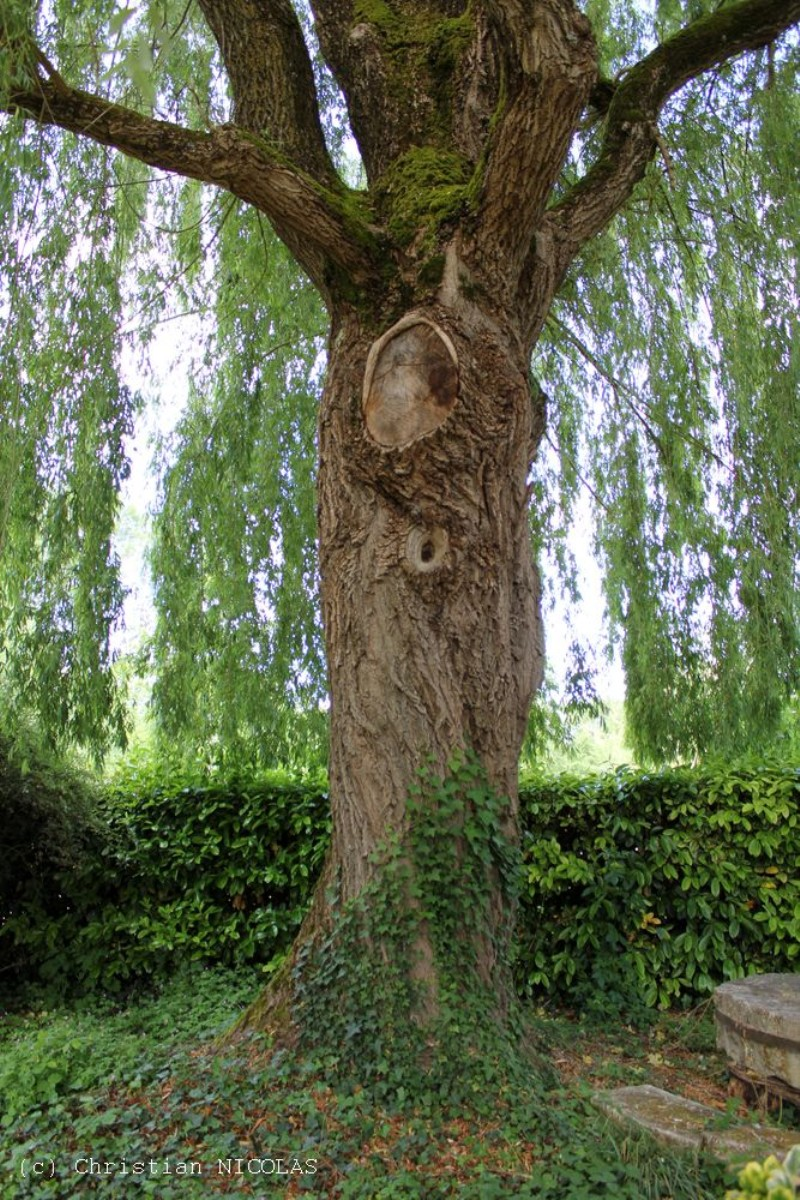
\includegraphics[scale=0.2]{gizeux-saule-pleureur-tronc.jpg}

Ne peut pas être supprimée
\end{center}
\end{frame}

\begin{frame}{Créer une nouvelle branche}
\begin{center}
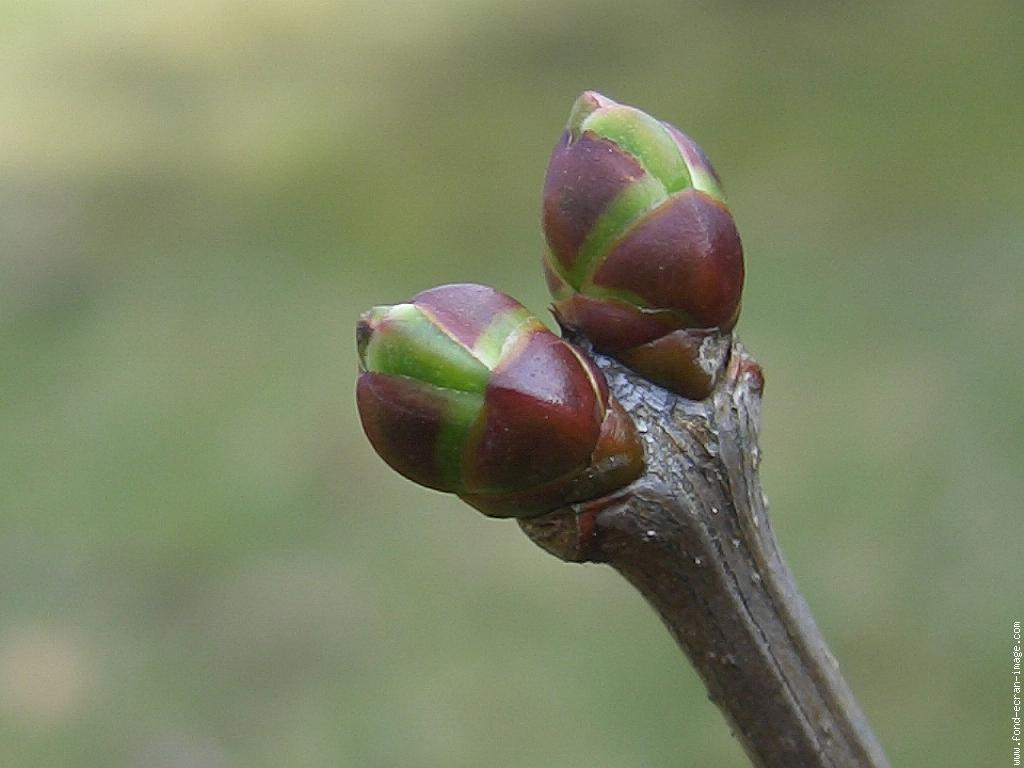
\includegraphics[scale=0.2]{bourgeons-3.jpg}

git branch ma-nouvelle-branche
\end{center}
\end{frame}

\begin{frame}{Se déplacer de branche en branche}
\begin{center}
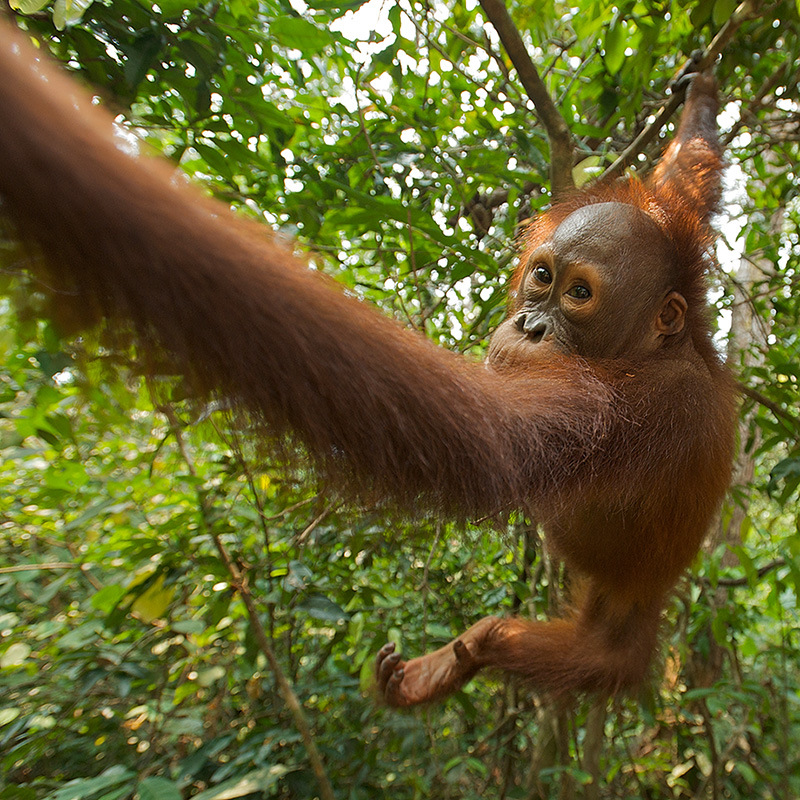
\includegraphics[scale=0.2]{orangutan_203x.jpg}

git checkout branche-a-atteindre
\end{center}
\end{frame}

\begin{frame}{Couper une branche}
\begin{center}
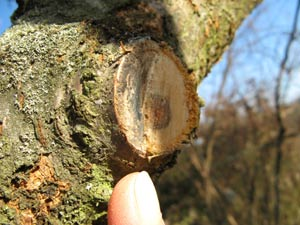
\includegraphics[scale=0.7]{scie-collet-branche.jpg}

git branch -d branche-a-couper
\end{center}
\end{frame}

\begin{frame}{Fusionner des branches}
\begin{center}

\includegraphics[scale=0.3]{Goten-Trunks-Fusion-dragon-ball-all-fusion-33379377-855-482.png}

git checkout branche-receptrice

git merge branche-source
\end{center}
\end{frame}

\begin{frame}{Identifiant de commit}
\begin{center}
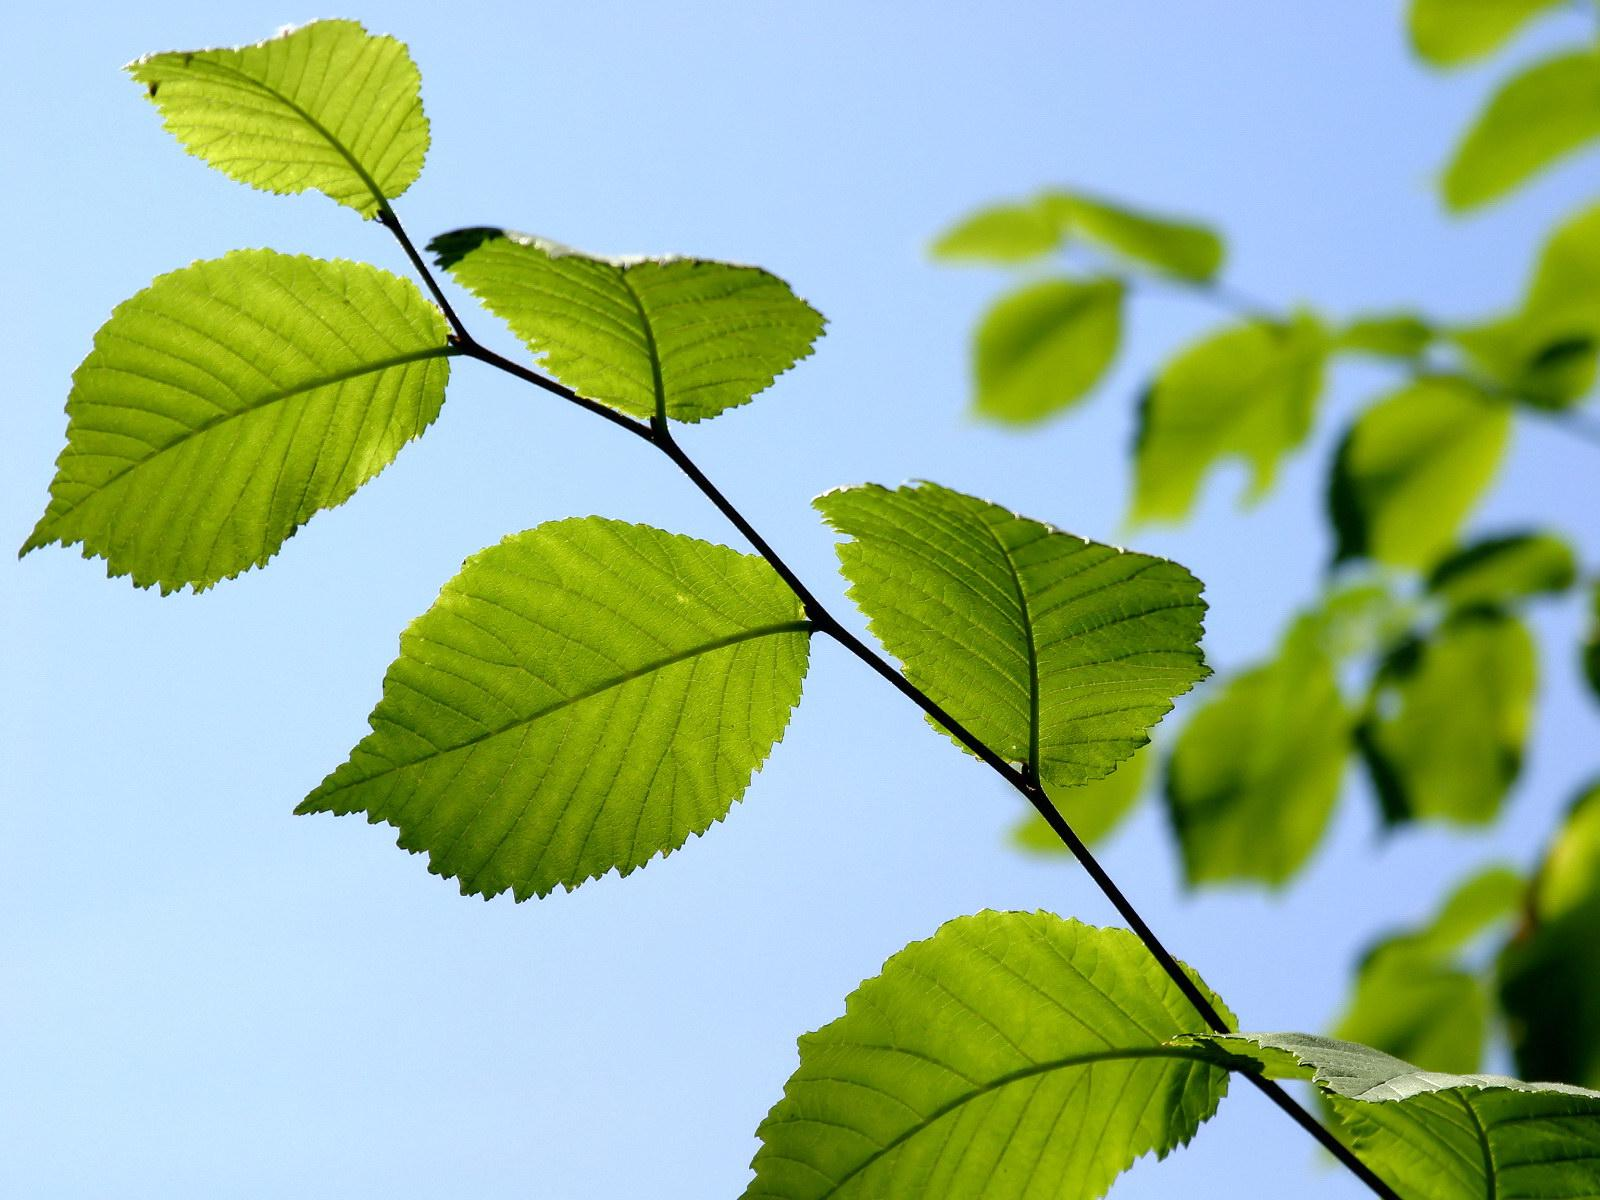
\includegraphics[scale=0.12]{feuille-arbre2.jpg}

Identifiant : hash de 160 bits (40 chiffres hexa)

Les 48 bits de poids fort suffisent (7 chiffres hexa)

HEAD est le dernier commit de la branche actuelle
\end{center}
\end{frame}

\begin{frame}{Revenir en arrière}
\begin{center}

\includegraphics[scale=0.17]{retour-vers-le-futur-85-02-g.jpg}

git reset --soft identifiant-du-commit (espace de travail inchangé)

git reset --hard identifiant-du-commit

git rebase --interactive identifiant-du-commit
\end{center}
\end{frame}

\begin{frame}{Rebaser une branche}
\begin{center}
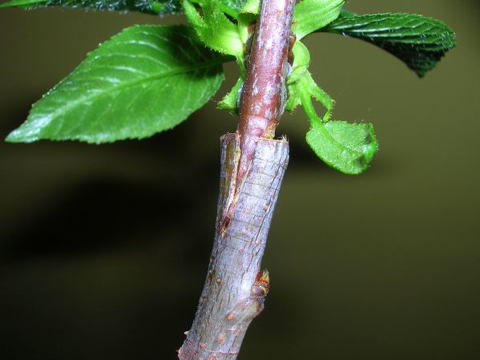
\includegraphics[scale=0.4]{greffe-00c1e2a50.jpg}

Remplace le commit de base de la branche

git checkout branche-a-rebaser

git rebase branche-sur-laquelle-rebaser
\end{center}
\end{frame}

\begin{frame}{Sources}
http://git-scm.com/book/fr/Les-branches-avec-Git-Brancher-et-fusionner\%C2\%A0\%3A-les-bases
\end{frame}
